\section{Testing}
\subsection{Frontend User Testing}
This section covers the informal user testing executed for front end usability and subsequent changes to the user interface. As suggested in our meetings we have carried out some informal testing on the target audience to get advice and feedback on our front end implementation. 

\subsection{Testing process}
As this as informal testing we recruited some volunteers from our target demographic i.e. CS students with little to no knowledge of time series analysis. With regards to the process we set the application to its default starting mode and allowed the user to navigate the application independently so that we could observe the application's level of intuitiveness. As the user navigates the site one of our team members monitored and made notes on comments they made as well as features that were overlooked. Once completed the user was asked for any further comments and suggested improvements in order to document their full experience.

\subsection{Results}
Some comments that were brought up during testing including the action taken to mitigate this.
\begin{enumerate}
\item 'Toolbar not obvious what to do even with instructions'. As a result, clearer steps were added in starting instructions that included references to the location of the settings i.e. in the top bar.
\item 'Signal configuration not obvious how to start'. In response to this, instructions were added underneath form heading to prompt user to select a signal type.
\item 'Even with notification on bookmark it is not completely clear what the use of it is'. In further development more explanation was added to the bookmark popover to indicate what the user could do with this URL and made note to emphasise the bookmark feature in the user manual as it is clear that its there but not what its used for.
\item 'Could have header to identify or brand application'. A clear header with the application name was added to the UI to give the user instant indication of the application use.
\item 'Signal parameters could have more explanation'. A modal with signal data indications was added for each type of signal to make it more clear for users. 
\item 'Confused about the combination bar'. As well as making it clear in the user guide what this is used for a tool tip was also added to warn users about combining signals other than sinusoids and trends using the product method. 
\end{enumerate}

\subsection{JavaScript Automated Testing}
This section details the automated test suites developed for the JavaScript portion of the application. 

If elected, these tests can be ran by any end-user with access to the source-code by entering the following command in a terminal launched from the directory: {\bf npm test}. This command runs all the test suites that Jest can find for the project and displays how many were successful and any errors or warnings that occur. 

\subsubsection{FileIO.js}
The following functionality has been tested for the File Uploading functionality of the application. 

\begin{enumerate}
    \item Verification of file prefix: This test checks that the {\bf fileTypeIsSupported(fileName)} method works as expected. The first test supplies a valid String filename, ending with a .csv prefix, and expects that the method will return 'true'.
    
    The next test supplies the same method with an invalid file name, {\it someInvalidFile.{\bf json}} and expects the method to return 'false'. This is because the file extension is not supported, hence we don't want it to return true for an unknown/unsupported file type.
    \item Verification of csv input to JavaScript Array: The first test creates a valid String of example csv test data (emulating real behaviour, as the {\it FileReader} object of {\bf parseFile()} method reads the csv as text.) A variable containing the expected output is then created below, but this time as a JavaScript array, and not encoded as a String object. The test then expects that, upon calling the {\bf csvToArray(csvData)} method with the supplied, valid csv string data, the method will return an object matching in structure to the expectedOutput variable created earlier.
    
    The following test then verifies that, upon being supplied with invalid, non-numerical csv data, an exception is thrown with the message {\bf Non-numerical data discovered in csv file.}
    
    Finally, the last test in this test suite verifies that csv data containing exponential values (formatted with e's and -'s) is successfully read and parsed by the class. Identical to the original test for parsing csv data, an String representation of some example csv test data is created along with an expected output as a variable containing a JavaScript array. The test calls the {\bf csvToArray(csvData)} method and expects to receive an object with a structure matching the expectedOutput variable created before.
\end{enumerate}

That concludes the automated testing for the FileIO module. You'll notice that there is no testing for 'reasonable' or 'sensible' data being uploaded to the application; the user should be able to experiment with the application however they see fit, and there should be as few guard rails as possible to prevent their exploration of these algorithms. 

\subsubsection{sessionStorage.js}
This section was a little trickier to test owing to the fact that the test requires a Browser's sessionStorage functionality in order to function correctly. As this test is running offline, absent a web browser, the sessionStorage functionality was initially very finicky and tricky to emulate/mock. Eventually a helpful library was discovered to emulate the sessionStorage functionality that integrated with Jest seamlessly; {\bf mock-local-storage}. As the name implies, this library mocks the local (\& and session) storage functionality of a web browser in the Jest framework. After the introduction of this library, testing was straightforward. 

Referenced within the tests of this helper class are a couple of constants required solely for testing: {\bf testKeyForSessionStorage} and {\bf validStringValue}. Both of these are relatively straightforward to comprehend: the first is the key which will be used to store the value of the object in session storage, the latter being the value to be stored.

The following is a record of how the functionality of this class was tested:
\begin{enumerate}
    \item Saving string to sessionStorage should succeed: As the name implies, this test verifies that upon saving an value to sessionStorage with this helper class with a given key, the data is, infact, stored in the browser's sessionStorage. 
    
    \item Saving JSON Stringified object should succeed and return valid string: This test ensures that an example JavaScript array, preserved and converted into a JSON String, can firstly be stored in sessionStorage, and secondly can then be retrieved without any corruption to the format of the JSON String. 
    
    \item Removing string saved in sessionStorage should succeed: This test removes the value associated with the given key in SessionStorage and verifies that upon requesting the value of the key afterwards, without rewriting a new value to the key, a {\it null} is returned. 
    
    \item Getting data from nonexistant key should return nothing: This test verifies that upon attempting to retrieve a value for a key which does not exist in sessionStorage (emulating behaviour of mis-typed parameter in code), the behaviour is safely handled and only a {\it null} reference is returned.
\end{enumerate}

\subsubsection{Application Frontend}
This section details the Jest tests corresponding to individual components responsible for the front-end functionality of the application.  

\begin{enumerate}
    \item {\bf graphs.test.js:} This component is responsible for ensuring that the graphs letting the user know the application is loading and awaiting the return of the STFT/EMD functions are correctly embedded within the HTML.
    
    Firstly, a template string block representing the loading graphs is declared as a constant to be referred to by the tests.
    
    The tests begin by firstly resetting the innerHTML of the document object to a default state. The area responsible for holding the chart within the page is also defined. 
    
    The initial test verifies that, after being instructed to display the loading graphs, the chart area of the web page updates itself to display the loading graphs.
    
    The next test ensures that the loading graphs are removed from the page upon given the instruction.
    
    \item {\bf infoPanel.test.js:} The infopanel component of the application is the side panel that protrudes when selecting either EMD or STFT for analysis. It contains information regarding how each anlysis method works, it's pros and cons. 
    
    The first test suite of this class verifies that the infoPanel is properly populated depending on the option being pressed, either STFT or EMD. Upon the user pressing either button, the info panel is populated with the corresponding information in it's method-name and method-info sections (for the sake of this test, they match the values created in a class mock constant), and that the matching button in the option-bar is darkened to reflect it has been selected. 
    
    The final test ensures that the infoPanel can be shown and hidden as required via the class associated with each tag in the document's inner HTML. 
    
    \item {\bf reset.test.js:} This component is responsible for returning the application to its default, starting state upon being called. 
    
    Before each test, the document.body.innerHTML is set to a simplified version containing a few buttons, a nav bar and some extra divs. This is just a stripped down version of the real HTML code that would be expected, which would be too large to fit succinctly within this test class.
    
    The first few tests ensure that the reset button can be enabled, rather than just remain in it's default greyed-out/disabled state, and that the opening message upon booting up the application can be shown/hidden upon request. These checks are all performed by checking the class associated with the HTML tag corresponding to the object in question.
    
    The last test verifies that the entire application resets properly upon the reset button being pressed: the opening message should be displayed, the reset signals button disabled, the STFT/EMD buttons to both be un-selected and the array object containing the signals to be generated is empty. 
    
    \item {\bf upload.test.js:} This class is responsible for handling the updating the user interface whenever a csv file is selected to be uploaded and parsed by the application. 
    
    The test verifies that upon the upload button being selected, the HTML for the upload file panel is being rendered and that the reset input signal button is enabled, allowing the user to reset the status of the application incase they've made a mistake.
\end{enumerate}

As a result of our unit testing the majority of the JavaScript code (Excluding configSignal.js and bookmark.js) has been auto-tested as demonstrated in our coverage reports. These reports also covered external imported modules used for the 'fileIO' module and therefore the overall coverage may be an underestimation for our developed code

\begin{figure}[H]
    \centering
    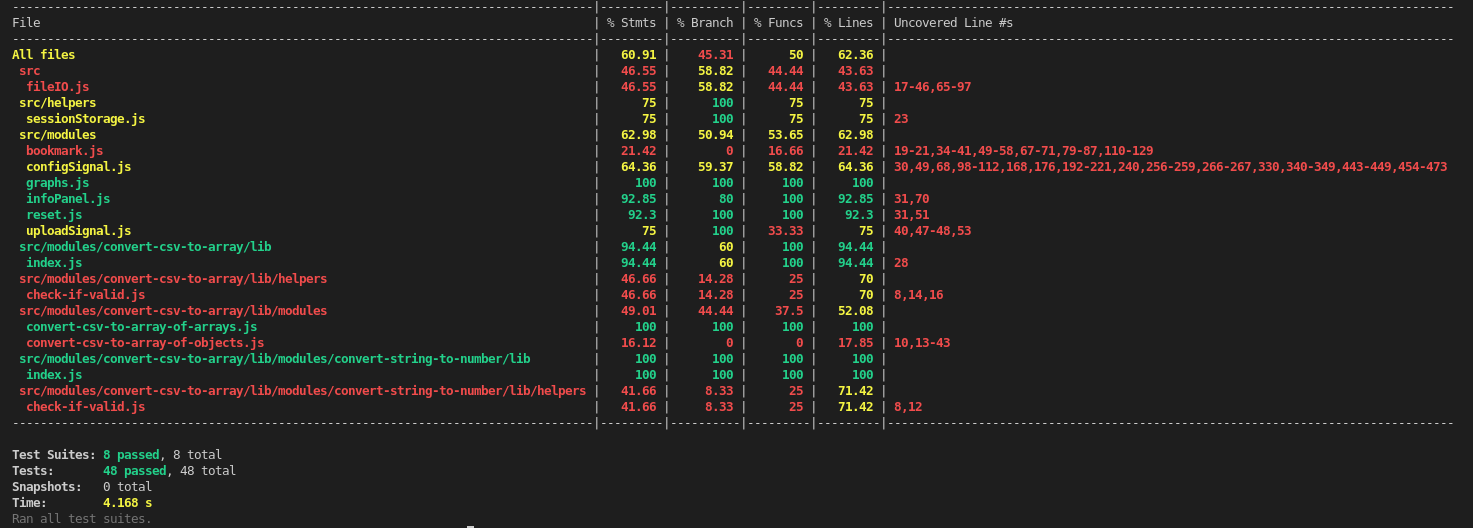
\includegraphics[width=1.0\textwidth]{figures/coveragereports.png}
    \caption{\label{fig:Coverage Report}Coverage Report}
\end{figure}


\subsection{JavaScript Manual Testing}
The frontend modules including 'bookmark.js', 'configSignal.js', 'graphs.js', 'infoPanel.js', 'reset.js' and 'uploadSignal.js' have been unit tested using Jest and the JSDOM plugin to some capacity though with time constraints and difficulties with mocking certain events and window objects 'bookmark.js' and 'config.js' do not have full function coverage in automated testing though they have all been manually tested through the common use cases which is outlined below.

\subsubsection{bookmark.js}
\begin{enumerate}
\item bookmarkToClipboard: This was checked through simply clicking on the bookmark button and checking if the current application URL was saved.
\item addParam, addSignalParam, removeSignalParam, editSignalParam: The tests for these involved checking the correct URL parameters were produced in the address bar of the browser. Additional comparison checks for ensuring the the URL parameter data is consistently passed to sessionStorage properly was also conducted. 
\item clearSignalParam, clearURLParam: These tests involved checking the URL again for the correct parameter clearance with test data.
\item paramsToObj: This takes the URL string and creates an object so in order to test this the URL was compared to the result of this function for any inconsistencies. 
\end{enumerate}

\subsubsection{configSignal.js}
\begin{enumerate}
\item displayDeleteBtn, displayAddBtn, displayEditBtn: These tests involved going through the common use cases of add, delete and editing signals to make sure the buttons appeared at the correct stages.
\item changeFormTemplate: This test was simply going through the different options of the select input on the signal configuration form and checking all the inputs are consistent with the signals schema that has been defined.
\item populateSettingsForm: This involved testing the edit functionality of the signals form as 
\item getEditSignalData: This was a intermediate function only used to edit the id of the signal data so it was simply tested by checking that the resultant signal data had a signal id that is consistent with the selected signal.
\item addSignalChip: This check was done visually as it creates a button to represent all the different signals, the page was also inspected to ensure the element was assigned the correct id.
\item getSignalData: This returns all the data from the signal form so test data was entered and checked for consistency through logs when the function was called.
\item addSignal: This function calls the addSignalChip function and increments the signal count as well as updating the session storage. This was tested through checking the signal count at different stages of adding signals and monitoring the session storage for changes.
\item showConfigureTab: This dynamically adds the elements of configure panel to the DOM using a template. This was tested visually through clicking on the tab button as well as checking the functionality of the different elements.
\end{enumerate}

\subsection{Python Manual Testing}
Because we lacked a CI/CD pipeline for this project, and there were conflicts encountered when attempting to test our Python code via Jest caused by Pyodide, we elected to simplify our testing for this portion of the application by reverting to manual testing, i.e. planning tests out methodically before writing our Python code, with expected outputs from a variety of reasonable \& edge case inputs. 

\subsubsection{Signal Generation}
With respect to the code base, the Signal Generation logic returns a series of data points in an array representing points of a time series; these points could refer to sinusoidal, financial, chrip etc., and on their own don't mean particularly much to a human reader. Instead, it was decided to write the code in a Jupyter notebook, and upon execution a graph to visualize the points would be created and embedded below the relevant code. An online graphing tool was then pulled up next to the Jupyter notebook window with the same graphing choices selected; the graphing functions were then verified sequentially by comparing the output of the Jupyter notebook with that of the online graphing tool. Any differences identified were analysed to pin-point where the fault in the logic was: for most cases, this was a simple case of mis-ordering the parameters of the graph. Upon correction, the graphs aligned identically, and it could be determined with relative certainty that the graph function was operating as intended.

\begin{figure}
    \centering
    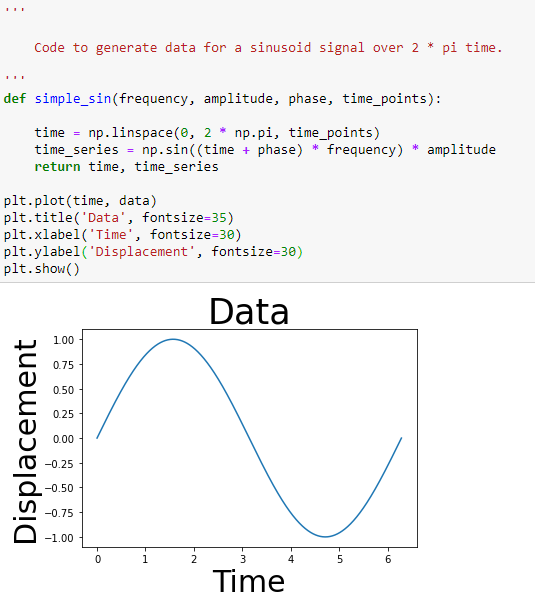
\includegraphics[width=280pt, height=280pt]{figures/jupyter.png}
    \caption{Example creation of a Sinusoidal wave image in the Jupyter Notebook test environment.}
    \label{fig:jupyter_test}
\end{figure}

The only signal types this testing strategy did not apply for were the coloured noise and poisson noise. This is because, as these graphs represent noise and hence involve randomness, consistent results across test runs couldn't be generated to compare with an online graphing tool (which, for these particular graphs, were rather tricky to come by.) 
Instead, it was decided to have faith in the {\it numpy} implementation of these functions, as numpy is a trusted library of numerous commercial \& enterprise applications, and to compare the outputs produced with examples of each type of noise found online (pink, brown etc.). Once a graph had been produced for each type of noise that matched an example found online, it was determined that the function worked correctly and any variance to the shape/format of the graph was caused by the inherent randomness involved noise generation function.

As mentioned in the design document, this application also offers the option of 'combining' multiple generated signals together, of different types and lengths, and analysing the resultant time-series via STFT/EMD analysis. This functionality was tested by creating an array of differing signal types spread out across (and overlapping one another) on a given time-frame (0 -\> 250ms, 249ms -\> 333ms, 300ms -\> 552ms ...) and firstly ensuring that a resultant time series would be generated, and secondly that the graph visualization made sense (e.g. there was a sinusoid where expected, followed by a chirp, followed by either the sum or product of a combination of a linear trend and chirp etc. etc.). Edge cases such as incomplete input, missing parameters and wildly different scales (e.g. utilizing seconds instead of milliseconds, amplitude/phase/frequency being 10x larger than other individual components) were all used to validate that a time series would be produced which could then be graphed. Once a time series was produced, it was then copied over and manually supplied to the STFT/EMD functions to verify that an analysis could be performed and a result was returned. 

Finally, once the manual testing had been completed for the individual Python functions, testing was performed on the communication between the JavaScript front-end and the Python code in the back-end. Simple tests were performed to verify that the generation options (what type of graph to produce, amplitude/frequency/phase etc.) were correctly stored in the Browser's session storage as a JSON object, that the options were being stored incrementally in an array rather than overriding a previously defined option and then that this JSON object could successfully be sent via Pyodide to the signal generation script and parsed into readable parameters to be executed by Python. 

Once all this had been accomplished, the signal generation component of the application was deemed to have been thoroughly tested and in a robust state, as no exceptions were being thrown and the resultant time series produced could then be analysed by the STFT/EMD analysis functions, meeting the criteria specified for the component. 

\subsubsection{EMD and STFT Analysis}

As noted in the design manual, this project utilizes 3rd party libraries to perform EMD and STFT analysis on a given time series; this choice was elected to minimize the time that would be taken to implement these algorithms from scratch and the overall robustness that could be assumed from a well-documented library.

The STFT implementation utilizes the {\bf signal.stft} functionality from the {\bf\href{https://scipy.org/}{Scipy}} library. To ensure that this implementation worked correctly, the {\bf\href{https://docs.scipy.org/doc/scipy/reference/generated/scipy.signal.stft.html}{Scipy STFT documentation}} was followed to verify that a graph matching the example embedded at the bottom of that guide was returned by our usage of the library. A class was created to generate custom, realistic time series' and parse into .csv format to emulate how the data would be handled by the application; for this specific test, a sample was generated matching the parameters of the example in the STFT function documentation. This time series was then parsed by the application to extract the time series data from the .csv file generated, supplied to the STFT analysis algorithm, the results plotted with mpld3 and the final graph compared to that in the documentation. Because they matched up perfectly, and tweaking the parameters of the time series generated still yielded sensible/expected results in the graphs generated, it was decided that the STFT implementation had been successfully tested. 

Due to the somewhat specialist \& niche nature of EMD analysis, there were fewer libraries to choose from to support this functionality; the following {\bf\href{https://emd.readthedocs.io/en/stable/index.html}{EMD Library}} was selected because of its thorough documentation which allowed for a similar testing strategy to the STFT implementation. After generating another batch of csv time series data locally using the similar parameters in the {\bf\href{https://emd.readthedocs.io/en/stable/emd_tutorials/00_quick_start/emd_tutorial_00_start_01_quicksift.html}{EMD Quick Start documentation}}, the time series data was parsed by the library and the resultant IMFs extracted (via the {\bf emd.sift.sift(x)} function.) The IMFs were then plotted with matplotlib and compared with the example in the documentation; because they aligned very closely (accounting for the minor changes in the time series structure due to how it was generated) it was decided that this library was satisfactory for use in the final application. 

To sum up the testing strategy for STFT/EMD analysis; for each library used, documentation was sourced with an example showing how to use the library. It was decided that because these algorithms produce graphs, a visual comparison was the best method of determining whether the results made sense rather than comparing the resultant plotting data with a static set of plot points, which also wouldn't work in the case of a time series being generated with random noise. A matching and/or similar time series would be supplied to the respective algorithm under test and the results would be graphed to allow for a visual comparison between what our implementation produced and that in the documentation. Once our csv test generation strategy was refined and our parameters supplied to each algorithm tweaked accordingly, matching graphs were being generated which meant we had faith that the implementation was working correctly. Sanity checks on the data would be performed earlier in the application to ensure appropriate data was being passed to these libraries, so our primary testing focus was to ensure that the results being returned made sense. 

\subsubsection{Pyodide}
Pyodide was tested extensively due to its integrity to the overall functionality of the application; without a working Pyodide implementation, there would be no way of communicating between the JavaScript front-end and the Python back-end to perform the signals analysis.
Although tested throughout development as front-end and back-end were gradually coupled together (which, as could be expected, resulted in greater overall stability and error-handling being implemented), there were a series of 5 feasibility tests conducted to assess the behaviour of Pyodide under different scenarios; these are as follows:

\begin{enumerate}
    \item {\bf Feasibility test 1:} An initial setup was created with numpy to generate a linear spread. A simple button was displayed on the front-end, and upon clicking it, Pyodide would be told to execute the numpy function in the back-end to calculate \& return a linear spread of values.
    
    Aside from gaining familiarity with Pyodide, the primary lesson learned was to avoid running signal analysis on the main thread as the page would lock-up and become unresponsive until the analysis was finished; the user may think that the application has stopped working and would restart their browser in response. 
    
    \item {\bf Feasibility test 2:} Similar to test 1, whereby a button clicked on the front-end would result in numpy generating a linear spread of numbers, however this time instead of executing on the main thread, a Web Worker thread was instantiated to handle the analysis.
    
    The lesson learned here was that the Web Worker prevents the page from becoming unresponsive as the main thread handling the user interface is no longer simultaneously performing the analysis with Python, however a downside was discovered that a Web Worker thread does not have access to the DOM. 
    
    \item {\bf Feasibility test 3:} Once again, a similar setup as before, however this time the results of the linear spread weren't returned to the front-end as a String, but rather they were converted into a graph by utilizing matplotlib, with the analysis and graph generation performed by a Web Worker. 
    
    It was discovered that matplotlib would annoyingly try to access a JavaScript package, which resulted in Pyodide being unhappy with this and killing the Web Worker thread when it calls for the JavaScript package. This was determined to be caused by Pyodide thinking that the Web Worker thread was attempting to access elements of the DOM. 
    
    \item {\bf Feasibility test 4:} A repeat of {\bf Feasibility test 3}, however this time matplotlib was instructed to use its Anti-grain geometry engine (AGG) instead of the default back-end. This is because the default back-end of matplotlib was what was making calls for a JavaScript package, whilst the AGG engine made no such calls.
    
    This test proved successful and allowed a graph to be generated by matplotlib and returned to the front-end via the use of a Web Worker instead of the main thread. 
    
    \item {\bf Feasibility test 5:} The final feasibility test, to ensure that parameters entered by the user on the front-end could be successfully captured and parsed by the Python back-end.
    
    The front-end used in the tests was tweaked slightly to add a text-box where a user could define the parameter used to generate the numpy linear spread. The analysis and graph generation were completed in the back-end by utilizing a Web Worker and matplotlib. 
    
    It was discovered that passing user parameters between the front-end and back-end was slightly trickier than previously thought due to JavaScript types and Python types not always being equivalent to one another, but a solution was identified as a result by wrapping the user-entered value in a String and then encoding this value in JSON. This value could then be parsed by the Python back-end without any issues as Python could infer the type from the JSON without needing to convert from JavaScript explicitly. 
\end{enumerate}

After incrementally testing this core functionality, and specifically understanding the limitations incurred with running Pyodide on the main thread and on a Web Worker respectively, as well as the type inference problems between JavaScript and Python, it was determined that Pyodide was suitable for the requirements of the project, and robust enough in it's implementation that so long as the Python code being executed in a Web Worker didn't call for a JavaScript package inside a Web Worker thread, it wouldn't crash when using compatible Python libraries such as numpy \& scipy, which were the primary libraries used for the signal generation and signal analysis classes.  

\section{Conclusion}
This concludes the test report for the application. As has been demonstrated above, a robust testing strategy has been utilized to ensure individual components were as expected. Suitable, reasonable edge cases have been chosen to test with, as has realistic/expected behaviour and the combination of the two has lead to a robust final product.

With more foresight, and a few less hiccups throughout development (specifically little niggles with Pyodide and sessionStorage), our Integration testing strategy would've relied less on manual testing by developers and could've been automated by either Jest or a python testing framework to further ensure end-to-end robustness of the application. Overall, the testing strategy proved effective and resulted in a stable \& usable final deliverable, even if a good portion of it was either done on-the-fly or incrementally whilst adding more complexity to a system component (i.e. Pyodide). The brief usability study which was conducted, although due to time constraints wasn't overly formal, allowed for valuable anecdotal feedback from the expected user demographic of the application on the front-end user interface, which was quickly incorporated to improve the usability of the application.  